%% Stellarium User Guide

\chapter{Deep-Sky Objects}
\label{ch:DSO}


Since version 0.10.0 Stellarium uses the ``json'' cataloguing system
of configuring textures. At the same time the Simbad online catalogue
was added to the search feature, making the catalog somewhat redundant
and used now only as a first search point or if there is no Internet
connection.

If the object has a name (not just a catalogue number), you should add
one or more records to the \file{.../nebulae/default/names.dat} file
(where \file{...} is either the installation directory or (preferrably) the user
directory). See section~\ref{sec:dso:modifyingNamesDat} Modifying
\file{names.dat} for details of the file format.

If you wish to associate a texture (image) with the object, you must
add a record to the \file{.../nebulae/default/textures.json} file. See
section~\ref{sec:dso:modifyingTexturesJson} for details.

If you wish to associate an outline with the object, you must add the
series of lines to the \file{.../nebulae/default/outlines.dat}
file. See section~\ref{sec:dso:modifyingOutlines} for details.


\section{Stellarium DSO Catalog}
\label{sec:dso:catalog}

Stellarium's DSO Catalog contains over 94000 objects\footnote{An extended edition of this catalog 
with over one million objects may be downloaded and installed manually (see section \ref{sec:ExtraData:DSOs}).} 
(up to $15.5^m$ for galaxies) and is available for end users as collection of files:

\noindent%
\begin{tabularx}{\textwidth}{lX}
%\emph{File} & \emph{Description}\\
\file{catalog.txt} &Stellarium DSO Catalog in ASCII format for editing data\\
\file{catalog.dat} &Stellarium DSO Catalog in zipped binary format for usage within Stellarium\\
\file{names.dat}   &List of proper names of the objects from file \file{catalog.dat}
\end{tabularx}

An edited ASCII file can be converted into binary format through enabling an option in the file \file{config.ini} (See \ref{sec:ConfigurationFile}):
\begin{configfile}
[devel]
convert_dso_catalog = true
\end{configfile}

The file \file{catalog.txt} should be put into the directory
\file{.../nebulae/default/} and you should create an empty 
file \file{catalog.pack} to storing the binary catalog. After converting the data into binary format 
you should gzip them by the command 
\begin{commands}
gzip -nc catalog.pack > catalog.dat
\end{commands}

Stellarium DSO Catalog contains data and supports the designations for
follow catalogs\footnote{Abell Catalog of Planetary Nebulae was added in v0.18.2 and removed in v0.20.1}:

\begin{description}[align=right,labelwidth=2cm]
\item[\textbf{NGC}]  New General Catalogue 
\item[\textbf{IC}] Index Catalogue 
\item[\textbf{M}] Messier Catalog
\item[\textbf{C}] Caldwell Catalogue 
\item[\textbf{B}] Barnard Catalogue~\citep{1927cdos.book.....B} 
\item[\textbf{SH2}] Sharpless Catalogue~\citep{1959ApJS....4..257S} 
\item[\textbf{vdB}] van den Bergh Catalogue of reflection nebulae~\citep{1966AJ.....71..990V} 
\item[\textbf{RCW}]  A catalogue of H$\alpha$-emission regions in the southern Milky Way~\citep{1960MNRAS.121..103R} 
\item[\textbf{LDN}]  Lynds' Catalogue of Dark Nebulae~\citep{1962ApJS....7....1L} 
\item[\textbf{LBN}]  Lynds' Catalogue of Bright Nebulae~\citep{1965ApJS...12..163L} 
\item[\textbf{Cr}] Collinder Catalogue~\citep{1931AnLun...2....1C} 
\item[\textbf{Mel}]  Melotte Catalogue of Deep Sky Objects~\citep{1915MmRAS..60..175M} 
\item[\textbf{PGC}]  HYPERLEDA. I. Catalog of galaxies\footnote{The PGC and UGC catalogs are partially supported}
\item[\textbf{UGC}]  The Uppsala General Catalogue of Galaxies
\item[\textbf{Ced}]  Cederblad Catalog of bright diffuse Galactic nebulae~\citep{1946MeLuS.119....1C}
\item[\textbf{Arp}]  Atlas of peculiar galaxies\footnote{Arp, VV and PK was added in version 0.16.0}~\citep{1966ApJS...14....1A}\newFeature{0.16.0}
\item[\textbf{VV}]  The catalogue of interacting galaxies by Vorontsov-Velyaminov~\citep{2001A&AT...20..717V}
\item[\textbf{PK}]  Version 2000 of the Catalogue of Galactic Planetary Nebulae~\citep{2001A&A...378..843K}
\item[\textbf{PN G}]  The Strasbourg-ESO Catalogue of Galactic Planetary Nebulae\footnote{PN G, SNR G and Abell was added in version 0.16.1}~\citep{1992secg.book.....A}\newFeature{0.16.1}
\item[\textbf{SNR G}]  A catalogue of Galactic supernova remnants~\citep{2014yCat.7272....0G}
\item[\textbf{Abell}]  A Catalog of Rich Clusters of Galaxies~\citep{1989ApJS...70....1A}
\item[\textbf{HCG}]  Atlas of compact groups of galaxies~\citep{1993ApL....29....1H}\newFeature{0.18.0}
\item[\textbf{ESO}]  ESO/Uppsala Survey of the ESO(B) Atlas~\citep{1982ESO...C......0L}\newFeature{0.18.2}
\item[\textbf{vdBH}]  Catalogue of southern stars embedded in nebulosity\footnote{vdBH and DWB was added in version 0.19.2}~\citep{1975AJ.....80..208V}\newFeature{0.19.2}
\item[\textbf{DWB}]  Catalogue and distances of optically visible H II regions~\citep{1969A&A.....1..270D}
\item[\textbf{Tr}]  Trumpler Catalog\footnote{Tr, St, Ru and vdB-Ha was added in version 0.20.2}\newFeature{0.20.2}
\item[\textbf{St}]  Stock Catalog
\item[\textbf{Ru}]  Ruprecht Catalog
\item[\textbf{vdB-Ha}]  van den Bergh-Hagen Catalog~\citep{1975AJ.....80...11V}
\item[\textbf{Other}] deep-sky objects without designations and sky regions\newFeature{0.20.3} --- by formal rules objects from this list are not included in any catalog known to Stellarium
\end{description}

\noindent Cross-index data for Stellarium's DSO Catalog is partially obtained from 
\citetp{2003A&A...399..141M} and astronomical databases 
SIMBAD\footnote{SIMBAD Astronomical Database --- \url{https://simbad.u-strasbg.fr/simbad/}}~\citep{2000A&AS..143....9W} 
and NED\footnote{NASA/IPAC Extragalactic Database (NED) --- \url{https://ned.ipac.caltech.edu/}}.

\noindent Distances for some deep-sky objects obtained from \citetp{2008ApJ...689..194S}, \citetp{2007ApJ...670..363H}, \citetp{1995A&AS..113..325H} and \citetp{1996AJ....112.1487H}.

\noindent Morphological class for many open clusters obtained from \citetp{1966BAICz..17...33R}.

\noindent Visual magnitudes for Messier objects obtained from ``Revised New General Catalogue and Index Catalogue'' by Dr. Wolfgang Steinicke (Version: 2 February 2021 --- NI2021)\footnote{Discovery and Cataloguing of Nebulae and Star Clusters --- \url{http://www.klima-luft.de/steinicke/index_e.htm}}.

\subsection{Modifying catalog.dat}
\label{sec:dso:modifyingCatalog.dat}

This section describes the inner structure of the files \file{catalog.dat}
(binary format) and \file{catalog.txt} (ASCII format).
Stellarium can convert ASCII file into the binary format file for faster usage
within the program.

Each line contains one record, each record consisting of the following
fields with \emph{tab} char as delimiter:

\begin{longtable}{r|l|p{110mm}}
\toprule
\emph{Column} & \emph{Type} & \emph{Description}\\\midrule
 1 & integer & Deep-Sky Object Identificator\\
 2 & float   & RA (decimal degrees)\\
 3 & float   & Dec (decimal degrees)\\
 4 & float   & B magnitude\\
 5 & float   & V magnitude\\
 6 & string  & Object type (See section~\ref{sec:dso:types} for details).\\
 7 & string  & Morphological type of object\\
 8 & float   & Major axis size or radius (arcmin)\\
 9 & float   & Minor axis size (arcmin)\\
10 & integer & Orientation angle (degrees)\\
11 & float   & Redshift\\
12 & float   & Error of redshift\\
13 & float   & Parallax (mas)\\
14 & float   & Error of parallax (mas)\\
15 & float   & Non-redshift distance (\Mpc\ for galaxies, \kpc\ for other objects)\\
16 & float   & Error of non-redsift distance (\Mpc\ for galaxies, \kpc\ for other objects)\\
17 & integer & NGC number (New General Catalogue)\\
18 & integer & IC number (Index Catalogue)\\
19 & integer & M number (Messier Catalog)\\
20 & integer & C number (Caldwell Catalogue)\\
21 & integer & B number (Barnard Catalogue)\\
22 & integer & SH2 number (Sharpless Catalogue)\\
23 & integer & vdB number (van den Bergh Catalogue of reflection nebulae)\\
24 & integer & RCW number (A catalogue of H$\alpha$-emission regions in the southern Milky Way)\\
25 & integer & LDN number (Lynds' Catalogue of Dark Nebulae)\\
26 & integer & LBN number (Lynds' Catalogue of Bright Nebulae)\\
27 & integer & Cr  number (Collinder Catalogue)\\
28 & integer & Mel number (Melotte Catalogue of Deep Sky Objects)\\
29 & integer & PGC number (HYPERLEDA. I. Catalog of galaxies); partial\\
30 & integer & UGC number (The Uppsala General Catalogue of Galaxies); partial\\
31 & string  & Ced identificator (Cederblad Catalog of bright diffuse Galactic nebulae)\\
32 & integer & Arp number (Atlas of Peculiar Galaxies)\\
33 & integer & VV number (The catalogue of interacting galaxies)\\
34 & string  & PK identificator (Catalogue of Galactic Planetary Nebulae)\\
35 & string  & PN G identificator (The Strasbourg-ESO Catalogue of Galactic Planetary Nebulae)\\
36 & string  & SNR G identificator (A catalogue of Galactic supernova remnants)\\
37 & string  & Abell identificator (A Catalog of Rich Clusters of Galaxies)\\
38 & string  & HCG identificator (Atlas of compact groups of galaxies)\\
39 & string  & ESO identificator (ESO/Uppsala Survey of the ESO(B) Atlas)\\
40 & string  & vdBH identificator (Catalogue of southern stars embedded in nebulosity)\\
41 & integer & DWB identificator (Catalogue and distances of optically visible H II regions)\\
42 & integer & Tr identificator (Trumpler Catalogue)\\
43 & integer & St identificator (Stock Catalogue)\\
44 & integer & Ru identificator (Ruprecht Catalogue)\\
45 & indeger & vdB-Ha identificator (Uniform survey of clusters in the Southern Milky Way --- van den Bergh-Hagen Catalogue)\\
\bottomrule
\end{longtable}

\subsubsection{Types of Objects}
\label{sec:dso:types}

Possible values for type of objects in the file \texttt{catalog.dat}.

\begin{longtable}{l|p{120mm}}
\toprule
\emph{Type} & \emph{Description}\\\midrule
G   & Galaxy\\
GX  & Galaxy\\
AGX & Active Galaxy\\
RG  & Radio Galaxy\\
IG  & Interacting Galaxy\\
GC  & Globular Cluster\\
OC  & Open Cluster\\
NB  & Nebula\\
PN  & Planetary Nebula\\
DN  & Dark Nebula\\
RN  & Reflection Nebula\\
C+N & Cluster associated with nebulosity\\
HII & HII Region\\
SNR & Supernova Remnant\\
SNC & Supernova Candidate\\
SNRC & Supernova Remnant Candidate\\
BN  & Bipolar Nebula\\
EN  & Emission Nebula\\
SA  & Stellar Association\\
SC  & Star Cloud\\
CL  & Cluster\\
IR  & Infra-Red Object\\
QSO & Quasar\\
Q?  & Possible Quasar\\
ISM & Interstellar Matter\\
EMO & Emission Object\\
LIN & LINEAR-type Active Galaxies\\
BLL & BL Lac Object\\
BLA & Blazar\\
MOC & Molecular Cloud\\
YSO & Young Stellar Object\\
PN? & Possible Planetary Nebula\\
PPN & Protoplanetary Nebula\\
$\ast$ & Star\\
$\ast\ast$ & Double Star\\
MUL & Multiple Star\\
SY$\ast$ & Symbiotic Star\\
EM$\ast$ & Emission-line Star\\
CLG & Cluster of galaxies\\
\emph{empty} & Unknown type, catalog errors, \emph{Unidentified Southern Objects} etc.\\
\bottomrule
\end{longtable}

\subsection{Modifying names.dat}%\label{modifying-names.dat}
\label{sec:dso:modifyingNamesDat}

Each line in the file \file{names.dat}  contains one record. A record
relates an extended object catalog number (from \file{catalog.dat})
with a name. A single catalogue number may have more than one record in
this file.

The record structure is as follows:

\noindent%
\begin{tabularx}{\textwidth}{r|r|l|X}
\toprule
\emph{Offset} & \emph{Length} & \emph{Type} & \emph{Description}\\
\midrule
0  &  5 & \%5s & Designator for catalog (prefix)\\
5  & 15 & \%d  & Identificator for object in the catalog\\
20 & 60 & \%s  & Proper name of the object (translatable)\\
\bottomrule
\end{tabularx}

\noindent If an object has more than one record in the file \file{names.dat},
the last record in the file will be used for the nebula label.

\subsection{Modifying textures.json}%\label{modifying-textures.json}
\label{sec:dso:modifyingTexturesJson}

This file is used to describe each nebula image. The file structure
follows the JSON format, a detailed description of which may be found
at \url{www.json.org}. The \file{textures.json} file which ships with
Stellarium has the following structure:

%% TODO: GZ notes 2016-04 It seems there is some overdocumentation here, some entries seem to repeat in this list. FIX THAT!

\begin{description}
\item[serverCredits (optional)] a structure containing the following
  key/value pairs:

  \begin{description}
  \item[short] a short identifier of a server where the json file is found, e.g. ``ESO''
  \item[full]  a longer description of a server, e.g. ``ESO Online Digitized Sky Survey Server''
  \item[infoURL] a URL pointing at a page with information about the server
  \end{description}
\item[imageCredits] a structure containing the same parts as a
  serverCredits structure but referring to the image data itself
\item[shortName] an identifier for the set of images, to be used inside Stellarium
\item[minResolution] minimum resolution, applies to all images in the set,
  unless otherwise specified at the image level
\item[maxBrightness] the maximum brightness of an image, applies to all
  images in the set, unless otherwise specified at the image level
\item[subTiles] a list of structures describing individual image tiles, or
  referring to another json file. Each subTile may contain:

  \begin{description}
  \item[minResolution]
  \item[maxBrightness]
  \item[worldCoords]
  \item[subTiles]
  \item[imageCredits]
  \item[imageUrl]
  \item[textureCoords]
  \end{description}
\item[shortName] (name for the whole set of images, e.g. ``Nebulae'')
\item[miniResolution] (applies to all images in set)
\item[alphaBlend] (applies to all images in set)
\item[subTiles] list of images. Each image record has the following properties:

  \begin{description}
  \item[imageCredits] (itself a list of key/pairs)
  \item[imageUrl] (e.g. file name)
  \item[worldCoords] (a list of four pairs of coordinates representing the corners of the image)
  \item[textureCoords] (a list of four pairs of corner descriptions. i.e. which is top left of image etc)
  \item[minResolution] (over-rides file-level setting)
  \item[maxBrightness]
  \end{description}
\end{description}

Items enclosed in Quotation marks are strings for use in the program.
Syntax is extremely important. Look at the file with a text editor to
see the format. Items in \textless{}\textgreater{} are user provided
strings and values to suit the texture and source.

\begin{configfileScr}
{
  "imageCredits"  : { "short" : "<author name>" , 
                      "infoUrl" : "http://<mysite.org>" 
                    }, 
  "imageUrl"      : "<myPhoto.png>",
  "worldCoords"   : [[[ X0, Y0], [ X1, Y1], [ X2, Y2], [ X3, Y3] ]], 
  "textureCoords" : [[[ 0,0],[1,0],[1,1],[0,1]]], 
  "minResolution" : 0.2148810463,
  "maxBrightness" : <mag>
},
\end{configfileScr}

where 

\begin{description}
\item[worldCoords] Decimal numerical values of the J2000 coordinates (RA and dec both in degrees) of the corners of the texture. These values are usually given to 4 decimal places.
\item[textureCoords]  Where 0,0 is South Left, 1,0 the South Right, 1,1 North Right, 0,1 North Left corners of the texture.
\item[minResolution] UNDOCUMENTED VALUE! Sorry!%% TODO FIXME!
\item[maxBrightness] total object brightness, magnitude 
\end{description}


Calculating of the coordinates of the corners of the images (plate solving) is
a time consuming project and needs to be fine tuned from the screen
display. As most images will be two dimensional, display on a spherical
display will limit the size to about 1 degree before distortion becomes
evident. Larger images should be sectioned into a mosaic of smaller
textures for a more accurate display.

\subsection{Modifying outlines.dat}
\label{sec:dso:modifyingOutlines}

\noindent\newFeature{0.16.1}Each line in the file \file{outlines.dat} contains three ``columns'' of data for outline elements. The structure for each line is as follows:

\noindent%
\begin{tabularx}{\textwidth}{r|r|l|X}
\toprule
\emph{Offset} & \emph{Length} & \emph{Type} & \emph{Description}\\
\midrule
0  &  8 & \%d  & Right ascension (decimal hours)\\
10 & 18 & \%d  & Declination (decimal degrees)\\
20 & 60 & \%s  & Command\\
\bottomrule
\end{tabularx}

\noindent Coordinates for each point of outline is represented in the equatorial coordinate system for epoch J2000.0. 
The possible values of the third ``column'' (\emph{Command}) are:
\begin{description}
\item[start] This command marks a start point of the outline. This command should also contain the designation of the deep-sky object.
\item[vertex] This command marks an intermediate point of the outline.
\item[end] This command marks an end point of the outline.
\end{description}


Example for outline of M42:
\begin{configfile}
05.56401 -05.49880 start  M 42 
05.56759 -05.39201 vertex 
05.56635 -05.31749 vertex 
05.57158 -05.21922 vertex 
05.57601 -05.21716 vertex 
05.58830 -05.30164 vertex 
05.59140 -05.34341 vertex 
05.59028 -05.37076 vertex 
05.59008 -05.38175 vertex 
05.59581 -05.37159 vertex 
05.59943 -05.47123 vertex 
05.59912 -05.65838 vertex 
05.59520 -05.73212 vertex 
05.58490 -05.68102 vertex 
05.56948 -05.57675 end
\end{configfile}

The format of the file \file{outlines.dat} is compatible with the similar file of the \program{SkyChart (Cartes du Ciel)} planetarium.

\section{Adding Extra Nebula Images}%\label{adding-extra-nebulae-images}
\label{sec:dso:adding_images}
\sectionauthor*{Glenn Newell}

\begin{figure}[htb]
\centering\includegraphics[width=\textwidth]{nebula-display.jpg}
\caption{Screen shot of nebula images displayed in Stellarium}
\label{fig:dso:adding_images}
\end{figure}

% Contributed 10/2019 for 0.19.3
\noindent In previous versions of this guide, the technique for preparing Deep
Space Object (DSO) images for inclusion in Stellarium involved \indexterm{plate
solving} the image to find its center on the sky, and then calculating
the corners of the image in the World Coordinate System (WCS\footnote{%
\url{https://fits.gsfc.nasa.gov/fits_wcs.html}}) using the scale of the
image, arc-seconds/pixel.


The problem with that approach is that it did not account for any
spatial distortion in the image, due to telescope optics or sensor
tilt, etc. This resulted in a labor intensive manual process of trial
and error to adjust the WCS corners of the image until the stars in
the image aligned with those displayed in Stellarium.

Fortunately, this problem has been solved for us by astronomers with
similar needs, extending \indexterm{FITS}\footnote{The \emph{Flexible Image
    Transport System} is the dominating image format used in
  astronomy.} file headers to include information on how
to map every pixel in an image correctly onto WCS coordinates. This
information can be added to your image when you plate solve it on
\program{nova.astrometry.net}, or similar services (local copies of
\program{astrometry.net}, such as \program{ansvr}, or in
\program{Pixinsight}, etc.). This system of correcting for distortions
in astronomical images was refined for the Spitzer
Space Telescope\footnote{\url{https://www.cs.helsinki.fi/group/goa/viewing/viewtransf/viewTrans.html}}.

It is now possible to utilize this pixel to WCS transformation data
included in plate solved images to prepare images for Stellarium that
map perfectly to the Stellarium sky without manual WCS corner
adjustments.

There are \program{Python} libraries, namely \program{astropy} and a
related ``channel'' \program{astroquery}, that can automate some or
all of the needed steps, and there are both manual and fully automated
scripts for that purpose available on Stellarium's GitHub site. These
scripts can be run on Windows, Mac, or Linux platforms, using the
\program{Anaconda Python} distribution.

\subsection{Image requirements for inclusion in Stellarium}
\label{sec:dso:adding_images:image-requirements}

The final image must be aligned with the equatorial (J2000.0)
coordinate system so that north is directly up and not inverted side
to side or up and down as can happen with photos taken with a diagonal
mirror in the path (In the WCS system, ``Parity'' must be 1.)

Next you will need to crop and/or re-scale the picture, setting the
main feature at the center and making the cropped size a power of 2,
e.g.\ 64, 128, 256, 512, 1024 or 2048 pixels square (or elongated like
$512\times1024$). If this requirement is not met, your textures may
not be visible, or graphics performance may be seriously impacted on
some systems. Textures larger than 2048 may only be supported on
high-end hardware. Images must be in PNG format. When cropping, make
sure you leave at least six prominent background stars for
\indexterm{plate solving}). The next step is to process your photo to
make the background black, really black. This will ensure that your
background will meld with the Stellarium background and not be noticed
as ugly gray square. Do not use ``transparent'' pixels available in
the PNG format as they will show as white, not black, in Stellarium.

Images covering more than 10 degrees of sky should be divided into
separate images, and images with pixel scales less than 1 arc-sec per
pixel should be re-scaled so as to have a pixel scale of 1 arc-sec per
pixel or larger.

\subsection{Processing requirements}
\label{sec:dso:adding_images:processing-requirements}

\begin{itemize}
\item \program{Python 3.7} (Anaconda 64~bit
  installer\footnote{\url{https://www.anaconda.com/distribution/}}) During
  installation, follow directions, taking defaults to install for
  just your user (vs.\ everyone on your computer)
\item \program{Astropy} (included in Anaconda)
\item \program{Astroquery} (latest version) To install on Windows,
  open an ``Anaconda Prompt''. On Mac and Linux, just open a
  terminal. At the prompt, enter:
  \begin{commands}
    pip install --pre --upgrade astroquery
  \end{commands}
\item For the fully automated process:
  \begin{itemize}
  \item An API Key from your account at \url{https://nova.astrometry.net}:
    \begin{itemize}
    \item Create an account (or log in with google, etc.) at \url{https://nova.astrometry.net}
    \item On the API tab, copy your API key (shown in green)
    \item Using a text editor (e.g., \program{Notepad++} on Windows,
      \program{Text Wrangler} on Mac OS), paste that key over the \texttt{X}'s
      in \file{Stellarium\_Nebulae\_Images\_Prep.py}'s
      \texttt{ast.api\_key = 'XXXXXXXXXXXXXXXX'}
    \end{itemize}
  \end{itemize}
\item For the more manual process: 
  \begin{itemize}
  \item Images plate solved at \url{https://nova.astrometry.net} (or \program{Pixinsight} -- not yet tested) so that WCS data is created
  \item Graphics software to flip, rotate, scale, etc. and save as \file{.png}, e.g., \program{Photoshop}, \program{GIMP}, \program{Pixinsight}, etc.
  \end{itemize}
\end{itemize}

\subsubsection{Script and Shortcut placement}

Download the Python scripts from Stellarium's site at Github\footnote{\url{https://github.com/Stellarium/stellarium-data/tree/master/adding-nebula-images}}:
\begin{itemize}
\item \file{WCS\_corners.py} script
\item \file{Stellarium\_Nebulae\_Image\_Prep.py} script
\end{itemize}
\begin{description}
\item[Windows]\mbox{}
  \begin{itemize}
  \item Place the two \file{.py} and \file{.bat} scripts into \file{\%USERPROFILE\%\textbackslash{}Anaconda3\textbackslash{}}
  \item Place the two Shortcuts on your desktop or an \file{astro tools} folder (optional)
  \item You can now drag and drop one or more images or \file{wcs.fits} files onto the shortcuts (or \file{.bat} scripts) for processing
  \end{itemize}
\item[Mac]\mbox{}
  \begin{itemize}
  \item Place the two \file{.py} script files in the \file{anaconda3} directory, which should be inside your home directory (the directory with your username).
  \item Place the two \file{.app} files on your desktop or an \file{astro tools} folder (optional)
  \item You can now drag and drop one or more images or \file{wcs.fits} files onto the \program{Automator} app icons for processing
  \end{itemize}
\item[Linux]\mbox{}
  \begin{itemize}
  \item Place the two \file{.py} script files in the \file{anaconda3} directory, which should be inside your home directory (the directory with your username).
  \item Place the two \file{.desktop} files on your desktop or an \file{astro tools} folder (optional)
  \item You can now drag and drop one or more images or \file{wcs.fits} files onto the desktop icons for processing
  \end{itemize}
\end{description}

\subsection{Manual processing}
\label{sec:dso:adding_images:manual}

We present the more manual of the two workflows and script first,
\program{WCS\_Corners.py}, so you understand the process, before
introducing the completely automated image processing pipeline. It is
also possible that if plate solving fails in the fully automated
script, you could continue, using this  manual process:

\begin{figure}[htbp]
\centering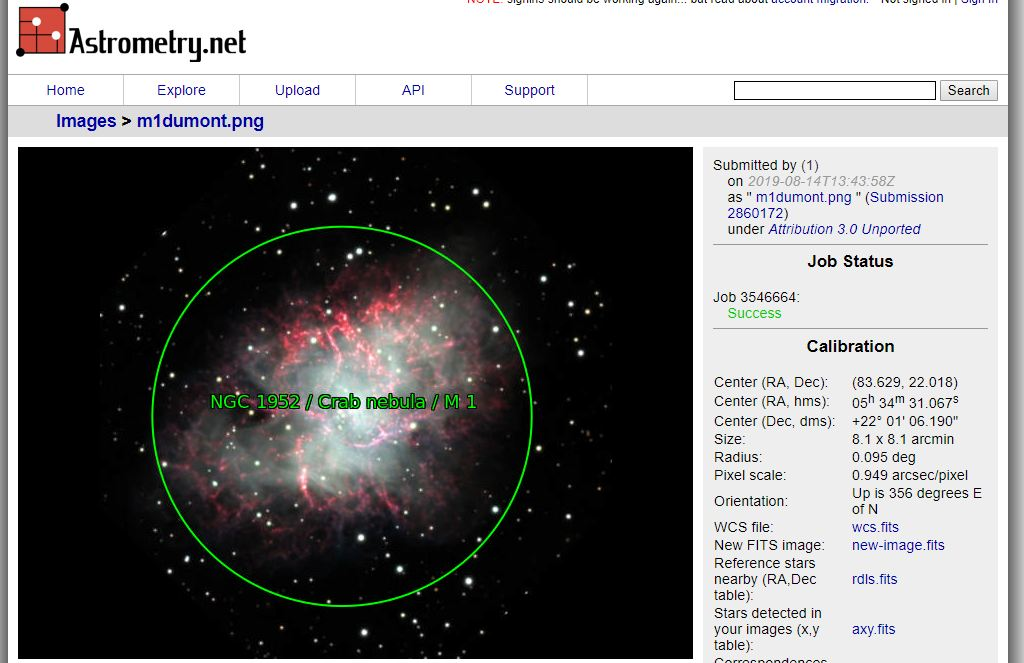
\includegraphics[width=\textwidth]{dso-add-1.jpg}
\caption{Online plate solving}
\label{fig:dso:adding_images:manual:plate-solving}
\end{figure}
\begin{figure}[htbp]
\centering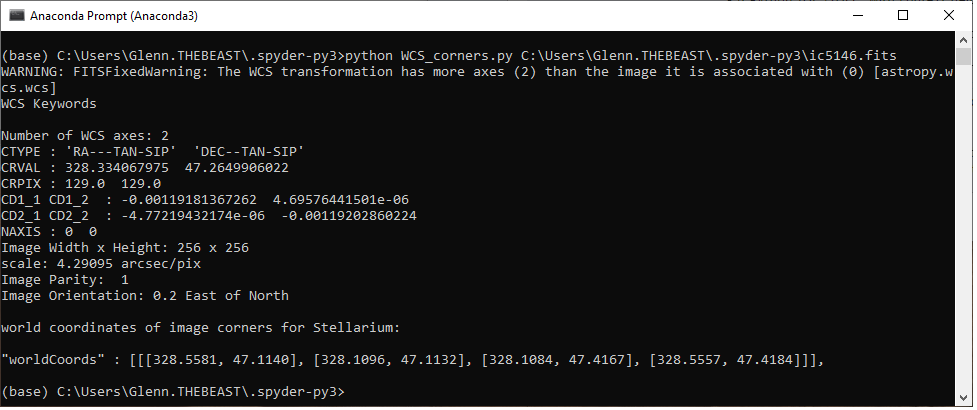
\includegraphics[width=\textwidth]{dso-add-2.png}
\caption{Python processing. If you just leave a space after \texttt{python WCS\_corners.py},
you can drag and drop your \file{wcs.fits} file into Windows' Anaconda Prompt window.}
\label{fig:dso:adding_images:manual:python}
\end{figure}

\begin{description}
\item[Plate Solve]\mbox{}
  \begin{itemize}
  \item Plate solve your image @ \url{nova.astrometry.net} (Fig.~\ref{fig:dso:adding_images:manual:plate-solving})
  \item Note \emph{pixel scale} and \emph{orientation}
  \end{itemize}
\item[Adjust Parity]\mbox{}
  \begin{itemize}
  \item Download the \file{wcs.fits} file from the ``Results'' page and run \program{WCS\_Corners.py} on it (Fig.~\ref{fig:dso:adding_images:manual:python}).
  \item If \emph{Parity} is -1, flip your image horizontally (do this before rotate step below)
  \end{itemize}
\item[Rotate]
  Rotate your image so ``up'' is exactly ``North''. i.e., if the orientation of your image was ``261 degrees East of North'' then rotate your image 261 degrees CW.
\item[``Blacken'' Sky]
  Fill in the blank areas of your rotated image with black pixels, and set your ``sky'' background to be black.
\item[Crop]
  Crop your image so that both $x$ and $y$ dimensions are powers of two pixels, e.g. $512\times512$, $1024\times1024$, $2048\times2048$, $1024\times2048$, etc.
\item[Save PNG]\mbox{}
  \begin{itemize}
  \item Save your image as \file{.png} file
  \item Place a copy into the \file{\%USERDIR\%/nebulae/default} directory
  \end{itemize}
\item[Plate Solve final image]\mbox{}
  \begin{itemize}
  \item Plate Solve your flipped, rotated, and cropped image again @ \url{nova.astrometry.net}
  \item Download the new \file{wcs.fits} file.
  \end{itemize}
\item[Calculate WCS corners]\mbox{}
  \begin{itemize}
  \item Run \program{WCS\_Corners.py} on the final \file{wcs.fits} file
  \item Edit Stellarium's \file{textures.json} with the image file name and the generated world coordinates
  \end{itemize}
\item[Finalize image]
  Try to minimize the number of stars visible around your nebula in your image. Stellarium draws its own stars, and a rectangle of excessive stars may look bad. Just blacken them out. 
\item[Restart Stellarium]
  View your image in Stellarium (and adjust \texttt{maxBrightness} in \file{textures.json} if needed)
\end{description}

%\newpage
Some additional information you should be aware of:
\begin{itemize}
\item Images in Stellarium are NOT tied to an object, just placed on the sky by \texttt{worldCoords}
  \begin{itemize}
  \item So multiple image can overlap. E.g., the bubble nebula has overlapping textures 
  \item Black is rendered transparent
  \item ``Transparent'' areas of \file{.png} show as white
  \end{itemize}
\item See section~\ref{sec:Directories} on Directories for where to put your own copy of the default images + yours, so yours won’t get overwritten by Stellarium Updates
\item If plate solve fails: adjust gamma/blackpoint so ``only'' stars are showing (Fig.~\ref{fig:dso:adding_images:manual:gamma})
\end{itemize}

  \begin{figure}[htbp]
    \centering
    \begin{tabular}{ccc}
      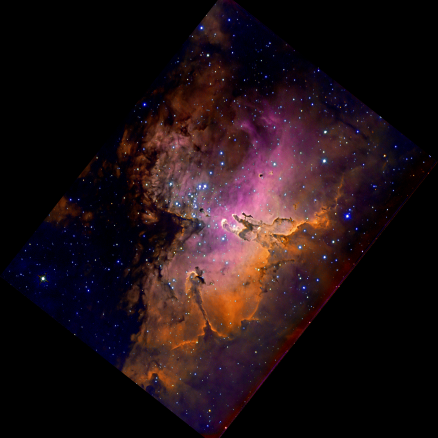
\includegraphics[width=0.38\textwidth]{dso-add-gamma1.png}&$\rightarrow$&
      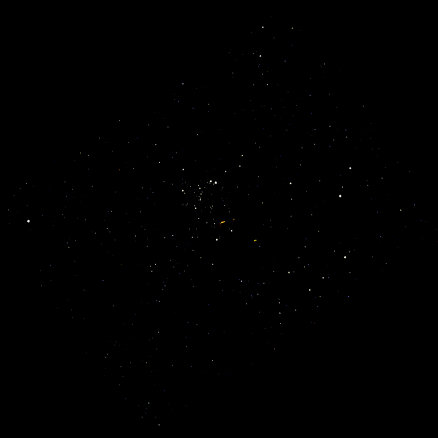
\includegraphics[width=0.38\textwidth]{dso-add-gamma2.png}
    \end{tabular}
\caption{Reduce gamma to temporarily help the plate solving algorithm finding stars.}
\label{fig:dso:adding_images:manual:gamma}
\end{figure}

  Stellarium keyboard shortcuts you may find useful when adding images:
  
\begin{tabular}{cl}
	\key{F3}&  brings up object search – Tab through search results\\
	\key{G} & to remove ground (in case your object is currently behind the landscape)\\
	\key{A} & to remove atmosphere  (in case it is daytime)\\
	\key{I} & to toggle nebulae images on and off – use to test star alignment\\
	\key{M} & to toggle Milky Way on and off\\
	\key{/} & to zoom into selected object\\
	\key{\textbackslash{}} & to zoom back out
\end{tabular}


\subsection{Automated processing}
\label{sec:dso:adding_images:auto}

\begin{figure}[tbp]
\centering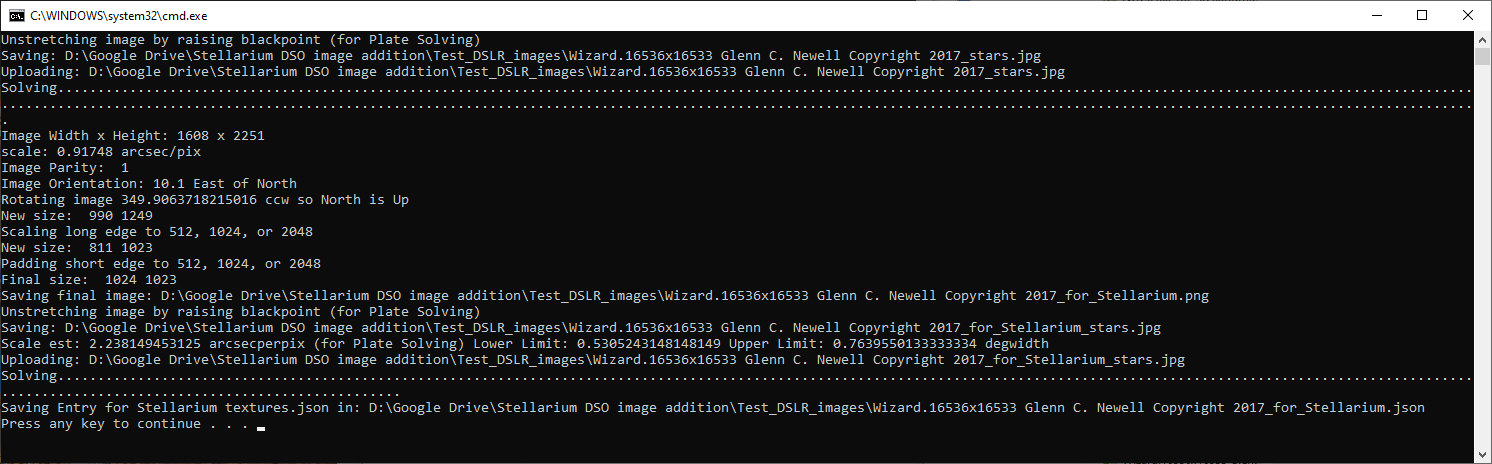
\includegraphics[width=\textwidth]{dso-add-auto-cli.png}
\caption{Automated Python processing with \program{Stellarium\_Nebulae\_Image\_Prep.py}}
\label{fig:dso:adding_images:auto}
\end{figure}

With the recent addition of \program{astrometry.net} queries to the
Python \program{astroquery} library it is now possible to automate
the entire image processing pipeline as well as automatically create
full \file{.json} entries for each image for inclusion in the
\file{textures.json} file. The python script for this is
\program{Stellarium\_Nebulae\_Image\_Prep.py}. Wrapper scripts
\program{Stellarium\_Nebulae\_Image\_Prep.bat} and
\program{Stellarium\_Nebulae\_Image\_Prep.sh} are also included so you
can process multiple images at once. With the desktop links you can even
process one or more \file{.jpg} or \file{.tiff} files by drag and
drop, on Windows, Mac, and Linux systems.

Figure~\ref{fig:dso:adding_images:auto} is an example run of
\program{Stellarium\_Nebulae\_Image\_Prep.py}.  This converts
(rotates, scales, etc.) the JPEG image as seen in
Fig.~\ref{fig:dso:adding_images:auto-result}, and a \file{.json} file
for inclusion in \file{textures.json}
(Fig.~\ref{fig:dso:adding_images:auto-json}), along with two
``unstretched'' \file{\_stars.jpg} images used for plate solving,
which can be deleted.

\begin{figure}[htbp]
  \centering
  \begin{tabular}{ccc}
    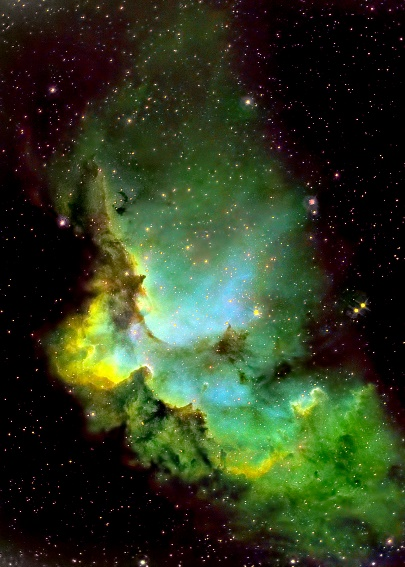
\includegraphics[height=5cm]{dso-add-auto1.jpg}&$\rightarrow$&
    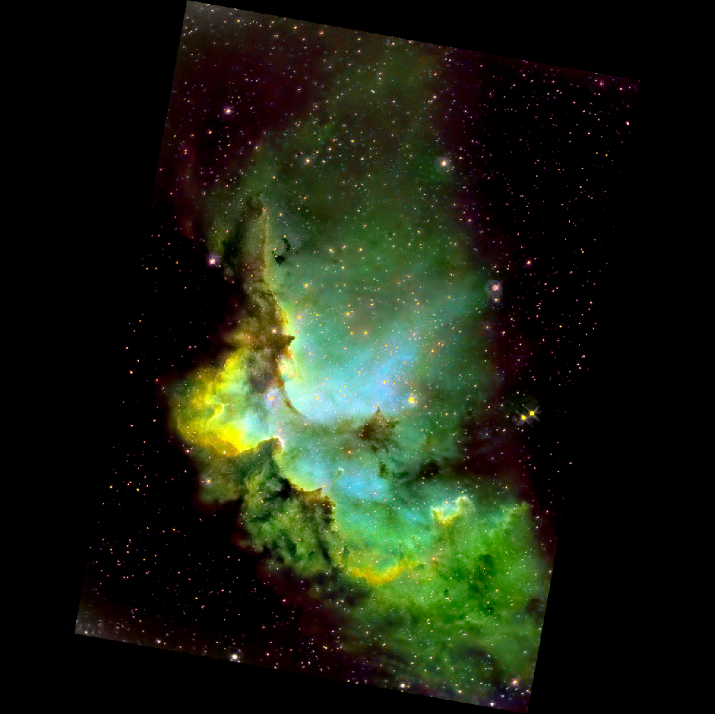
\includegraphics[height=5cm]{dso-add-auto2.png}
  \end{tabular}
  \caption{Automatic processing of a DSO image.}
  \label{fig:dso:adding_images:auto-result}
\end{figure}
\begin{figure}[htbp]
\centering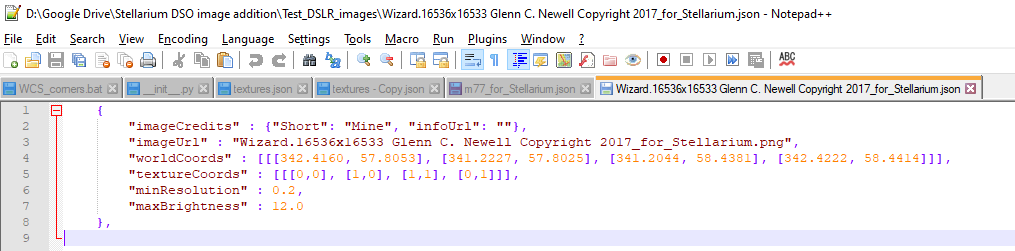
\includegraphics[width=\textwidth]{dso-add-auto-json.png}
\caption{\file{.json} result from processing with \program{Stellarium\_Nebulae\_Image\_Prep.py}}
\label{fig:dso:adding_images:auto-json}
\end{figure}

\subsection{Troubleshooting}


If no images show up in Stellarium, chances are you have introduced
one or more errors in the \file{textures.json} file.  You can use
\program{Json Lint} \footnote{An online service available at
  \url{https://jsonlint.com/}} to check for problems.

Just paste the entire contents of the file in and press ``Validate JSON''.

However, the original  \file{textures.json} file as shipped in v0.19.1 also fails:
\begin{itemize}
\item Missing leading zeros in front of decimal points
\item White space (a tab in this case) before \texttt{http} in \texttt{infoUrl} entries
\end{itemize}
These minor issues seem however not to irritate Stellarium.


% %%%%%%%%%%%%%%%% OLD INSTRUCTIONS. Delete when the new instructions are fully integrated.
\iffalse 
\sectionauthor*{Barry Gerdes}

\subsection{Preparing a photo for inclusion to the \texorpdfstring{\file{textures.json} file}{textures.json file}}
\label{sec:dso:preparing-a-photo}

\begin{figure}[h]
\centering\includegraphics[width=\textwidth]{nebula-display.jpg}
\caption{Screen shot of nebula images displayed in Stellarium}
\label{fig:dso:preparing-a-photo}
\end{figure}

The first step is to take a photo of the object you wish to display in
Stellarium. When you have the picture you will need to align it with
the equatorial coordinate system so that north is directly up and not
inverted side to side or up and down as can happen with photos taken
with a diagonal mirror in the path. Next you will need to crop the
picture, setting the main feature at the centre and making the cropped
size a factor of $2^n$ eg. 64, 128, 256, 512, 1024 or 2048 pixels
square (or elongated like 512x1024).  If this requirement is not met,
your textures may not be visible, or graphics performance may be
seriously impacted. Textures larger than 2048 may only be supported on
high-end hardware. Images must be in PNG format.  When cropping, make
sure you leave at least six prominent background stars.

The next step is to process your photo to make the background
black, really black. This will ensure that your background will meld with the
Stellarium background and not be noticed as gray square. Suitable programs to do all
this are \program{The GIMP}\footnote{free in keeping with the Stellarium spirit; available from \url{https://www.gimp.org}} or
\program{Photoshop} if you can afford it.

When you have your image prepared you will need to plate solve it using
at least 6 known GSC stars that can be identified. That is why the
cropping with plenty of stars was necessary. When the plate is solved
you will need to find the J2000 coordinates of the corners and convert
them to decimal values to form the world coordinates in the
\file{textures.json} file.

\begin{figure}[tb]
\centering\includegraphics[width=\textwidth]{EQ-Decimal.jpg}
\caption{\program{Stellarium Textures Generator}: A program to convert Equatorial coordinates into decimal
form and write a \texttt{textures.json} insert}
\label{fig:dso:STGen}
\end{figure}

The program \program{Stellarium Textures Generator} by Peter Vasey (Fig.~\ref{fig:dso:STGen}) can convert the corner coordinates of a
texture found in your plate solving program into decimal values and write an
insert for the \file{textures.json} file.\footnote{It is available as a freebee
from
\url{http://www.madpc.co.uk/~peterv/astroplover/equipnbits/Stellariumtextures.zip}.}

\begin{figure}[t]
\centering\includegraphics[width=\textwidth]{pix-4.jpg}
\caption{\program{ReadDSS}: A program to write a \file{textures.json} insert with epoch manipulation.}
\label{fig:dso:ReadDSS}
\end{figure}

There is another program, \program{ReadDSS} (Fig.~\ref{fig:dso:ReadDSS}), written by Barry Gerdes in Qb64(gl), that will perform the same
task but allows manipulation of the epochs.\footnote{
\url{http://barry.sarcasmogerdes.com/stellarium/uploads/writejsoninsert.zip}}

Another workflow was presented in the Stellarium forum on
SourceForge\footnote{\url{https://sourceforge.net/p/stellarium/discussion/278769/thread/60dfac82/#6a6d}}.

\subsection{Plate Solving}%\label{plate-solving}
\label{sec:dso:plateSolving}

Suitable programs that can accept your picture and calculate its corner
coordinates are hard to find. I have only found one that suits our
purpose and it is another expensive planetarium program, \program{TheSky X Pro}.
However the older versions \program{TheSky 5} and \program{6 Pro} will also do the job if
suitably configured, although I could not solve the test program with 
\program{TheSky 6} that uses the same procedure as \program{TheSky 5}.

These programs have a link feature that can match your photo to the
selected area of the screen and superimpose it on the display with a box
around your photo provided it can match at least 6 stars from the GSC
that is included with the program. When this is fitted you can read the
corner coordinates of your texture in the Status bar by selecting them
with a mouse. \program{TheSky X} can read these coordinates in J2000 values and
uses textures in the FITS format, but the earlier programs only read the
coordinates of the current program date. To read the J2000 coordinates
it is necessary to re-start the program with the date set to 1-1-2000.

To add the picture to \program{TheSky 5} you need first make a mono 8 bit version
of the photo and place it on the clipboard. Run \program{TheSky} and centre on the
object centre. Look in the \menu{Tools} menu for the \menu{image} link and select
\menu{setup}. Tick \menu{show image frame} to put a frame around the image.

Paste the clipboard image on the display and use the zoom and position
controls to get it as close to the size and position as possible by
visually matching stars. Go to the menu again and click on \menu{link wizard}.
If you have been successful the window will show the number of stars
matched and the option to \menu{accept} or \menu{continue}. Accept and you will now
see all the matched stars have overlaid the picture. You can now read
off the corner coordinates from the status bar starting at the bottom
(south) left and continuing counterclockwise to the top (north) left.

\subsection{Processing into a \texorpdfstring{\texttt{textures.json} insert}{textures.json insert}}%\label{processing-into-a-textures.json-insert}

Place your image in the \file{*.png} format in the
\file{.../nebulae/default/} folder. Ensure that the name matches the
\file{textures.json} entry.

Once you have the corner coordinates of your photo you can add them to
the decimal converter program and it will write an insert
\file{nebula.json} as a text file that you can paste directly into the
\file{textures.json} file that is in the \file{.../nebulae/default/}
folder.

Save the \file{textures.json} file with the new insert and run
Stellarium. Find the object in the \key{F3} Object selection window and slew to
it. Your image should be there and with a bit of luck it will nicely
overlay the stars in Stellarium. However this only rarely
happens, so a little bit of tweaking of the JSON \parameter{worldcoords} will be
needed to get a perfect match. Select equatorial mode (\guibutton{0.6}{bt_coord_type.png} or \keys{\ctrl+M}).
This will show the area with north up. Select each corner in sequence
and make small changes to the coordinates. Restart Stellarium each time
and check if you have moved into the right direction. Continue with each
corner until all the stars match. With a little bit of practice this
will be done in about 10 minutes.
\fi
% %%%%%%%%%%% OLD INSTRUCTIONS END


%%% Local Variables: 
%%% mode: latex
%%% TeX-master: "guide"
%%% End: 
